\subsection{Nuove funzionalità}

\setLayout{vertical}
\begin{frame}
    \frametitle{Nuove funzionalità}
    Abbiamo aggiunto funzionalità nuove rispetto a quelle dell'interfaccia originale: per la loro scelta abbiamo fatto riferimento alle esigenze e preferenze che ci hanno manifestato i giornalisti.\\
    Esse sono:
    \begin{itemize}
        \item \hyperlink{f:custom}{\textbf{Personalizzazione del contenuto informativo}}
        \item \hyperlink{f:pop}{\textbf{Pop-up di aggiornamento}}        
    \end{itemize}

\end{frame}

\begin{frame}
    \frametitle{Personalizzazione del contenuto informativo}
    \label{f:custom}
    Nell'intestazione delle schermate, abbiamo inserito un bottone chiamato "Seleziona metriche", al cui clic compare la lista delle metriche disponibili per la schermata corrente, ognuna delle quali può essere trascinata all'interno della schermata stessa, in sostituzione di una componente preesistente. 
    \vspace{-30pt}
    \begin{alertblock}{Miglioramento ottenuto}
        In questo modo è stato possibile incrementare la capacità informativa della dashboard, senza sacrificare la leggibilità di ogni componente grafica.        
    \end{alertblock}

\end{frame}

\begin{frame}
    \frametitle{Personalizzazione del contenuto informativo}
    \begin{figure}
        \centering
        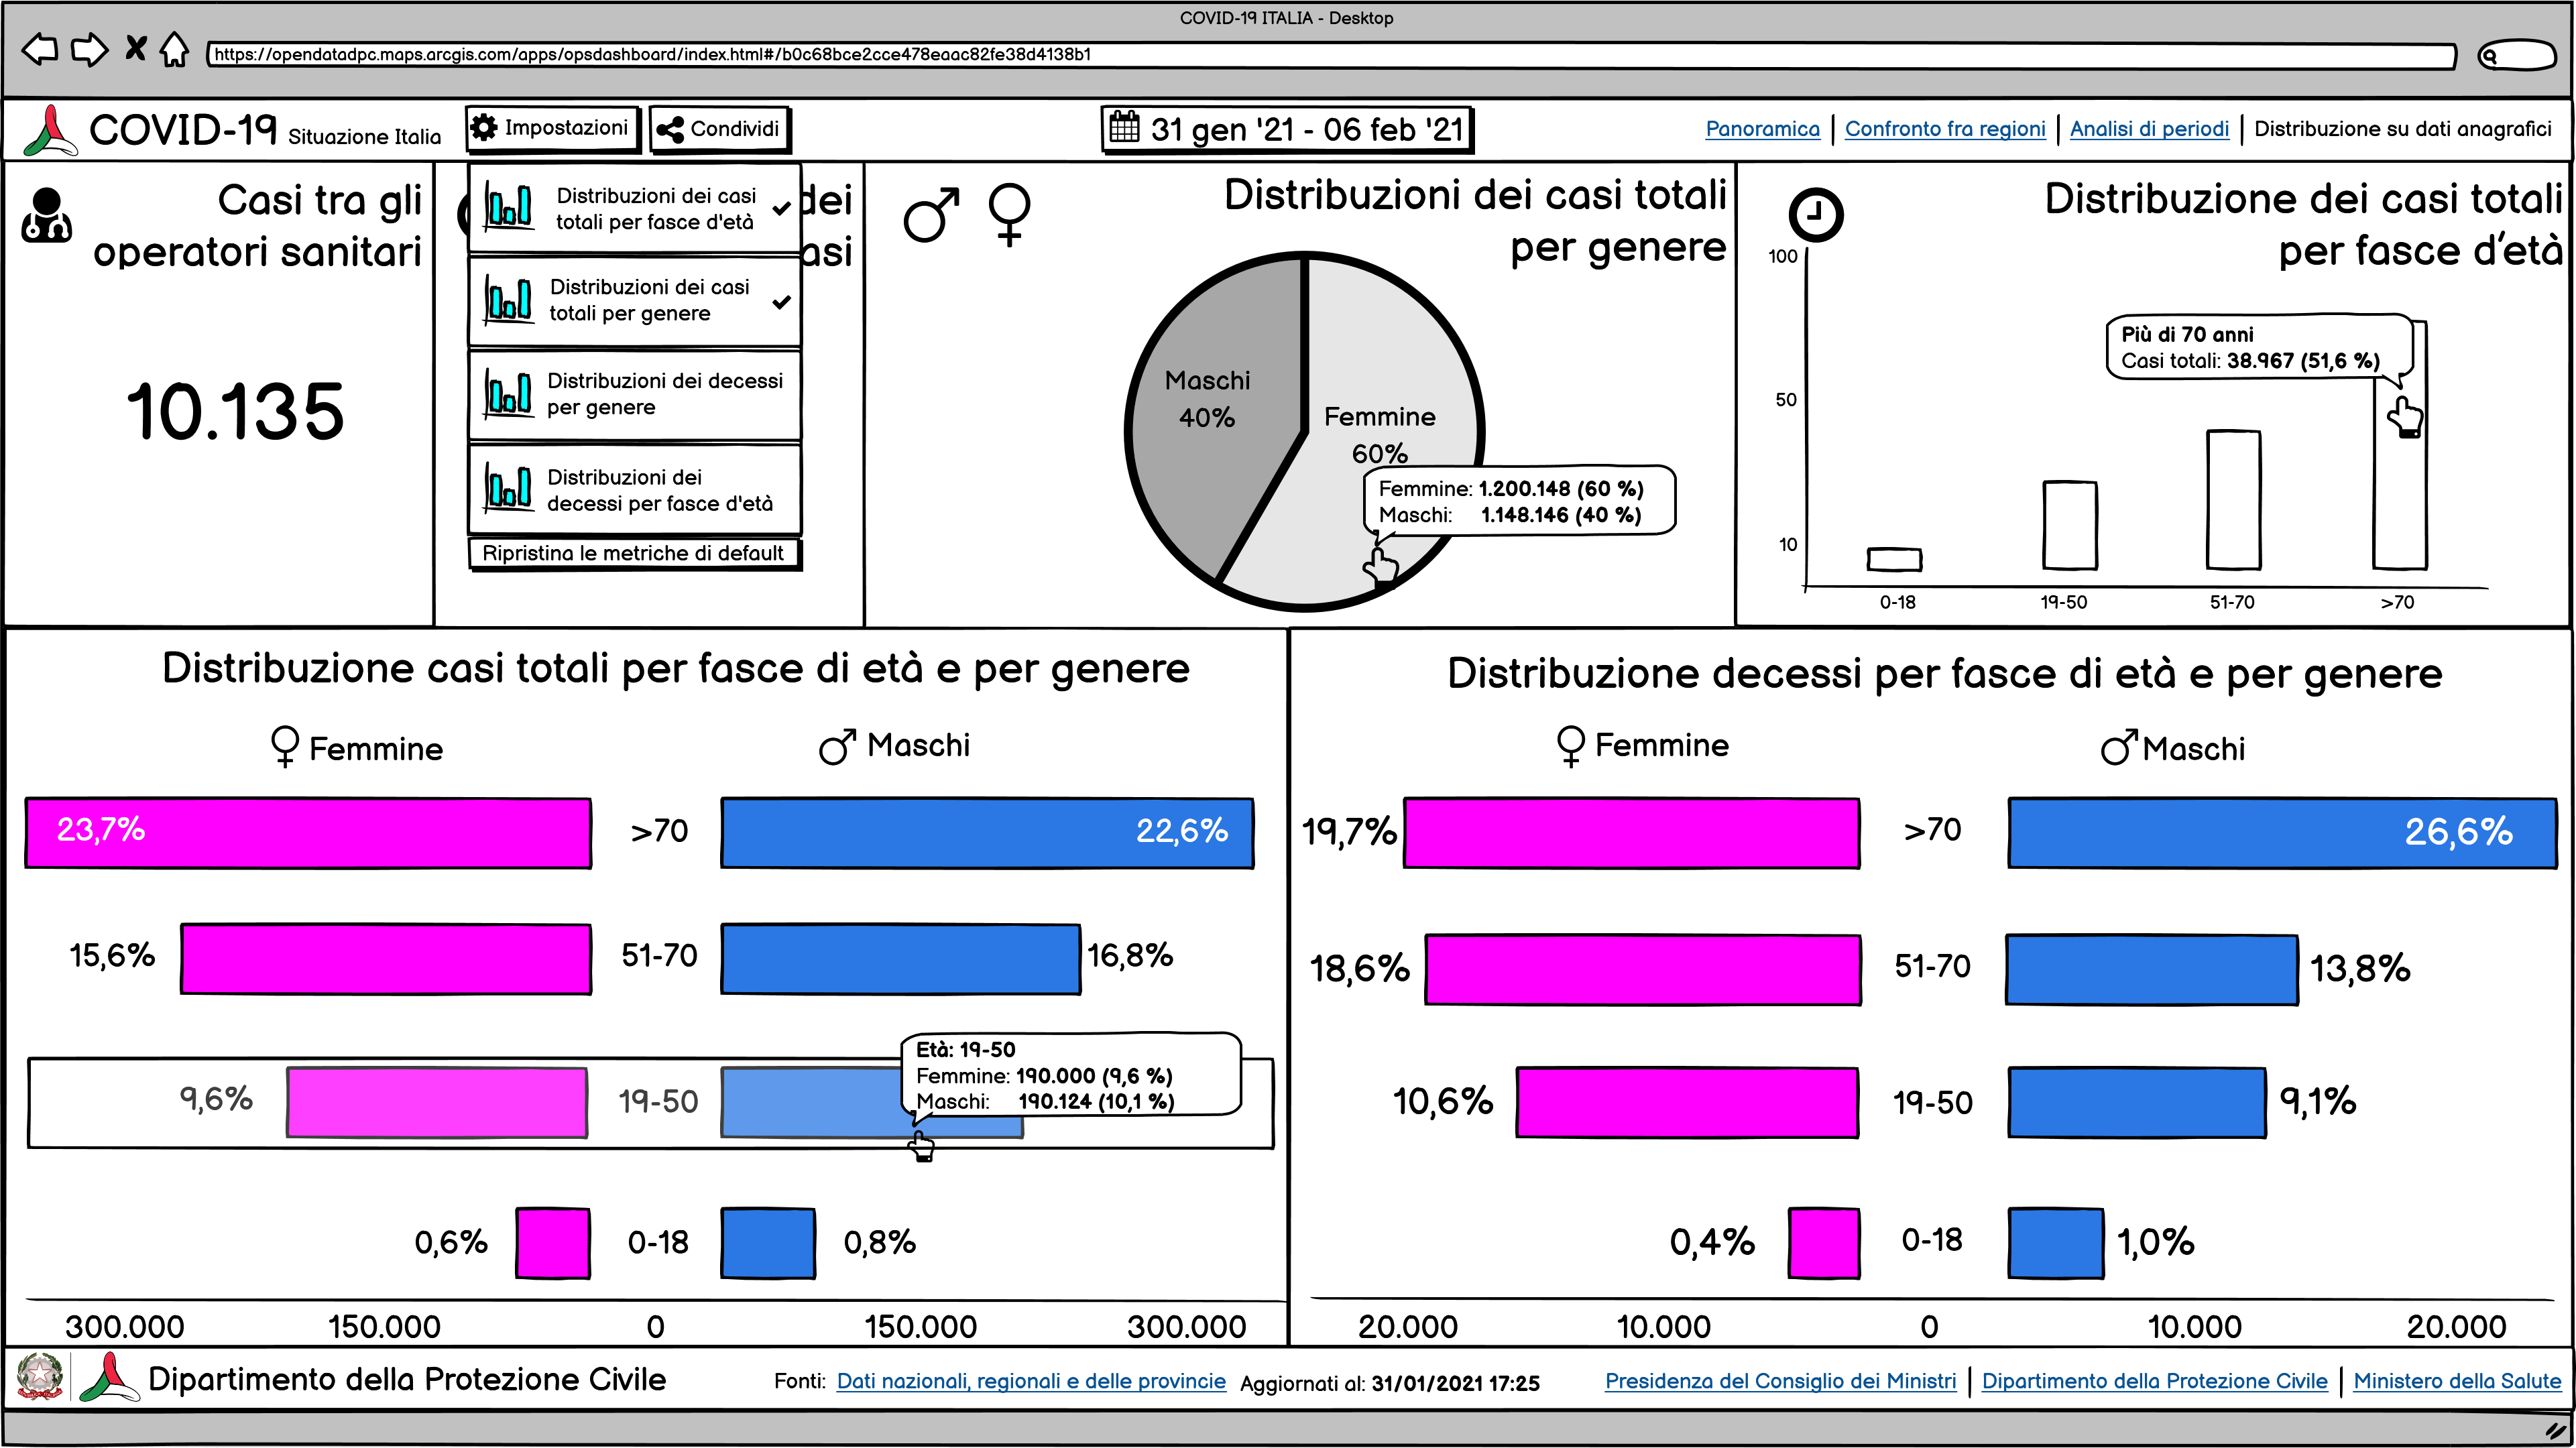
\includegraphics[trim = 0 20 0 55, clip, width=.8\textwidth]{screen-interfaccia/2 - Distribuzione su dati anagrafici.png}
        \caption{Schermata "Distribuzione su dati anagrafici" con "Impostazioni" aperto.}
    \end{figure}

\end{frame}

\begin{frame}
    \frametitle{Pop-up informativo}
    \label{f:pop}
    Per segnalare all'utente che sono disponibili i dati del giorno corrente, compare a schermo un pop-up informativo: l'autorizzazione per la sua comparsa è richiesta alla prima apertura della dashboard, come mostrato nella \hyperlink{fig:autoriz}{figura} della slide seguente.
    \vspace{-30pt}
    \begin{alertblock}{Miglioramento ottenuto}
        Quotidianamente, i nuovi dati sono pubblicati tra le 17 e le 19: grazie al pop-up informativo, l'utente può aprire la dashboard alle 17 e continuare i propri task tranquillamente, senza dover aggiornare la pagina continuamente.       
    \end{alertblock}

\end{frame}

\begin{frame}
    \frametitle{Pop-up di aggiornamento}

    \begin{columns}
        
        \column{.4\textwidth}
        \begin{figure}
            \centering
            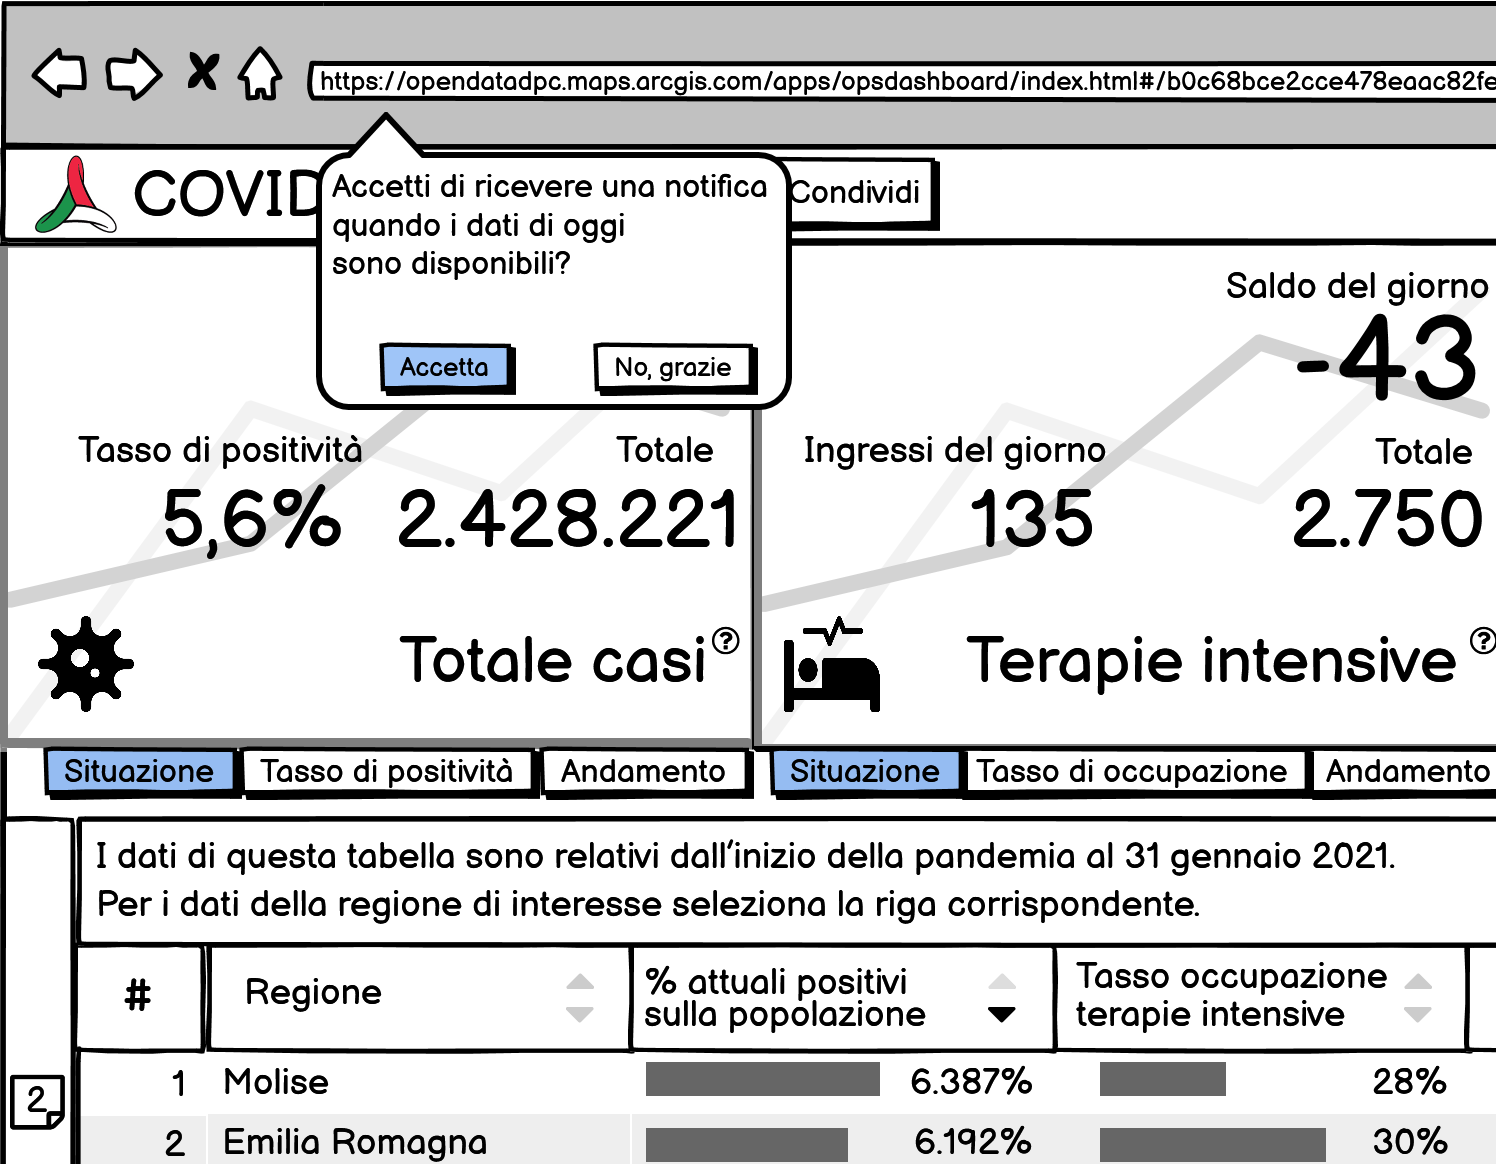
\includegraphics[width=\columnwidth]{screen-interfaccia/autor.png}
            \caption{Richiesta dell'autorizzazione a inviare notifiche.}
            \label{fig:autoriz}
        \end{figure}

        \column{.4\textwidth}
        \begin{figure}
            \centering
            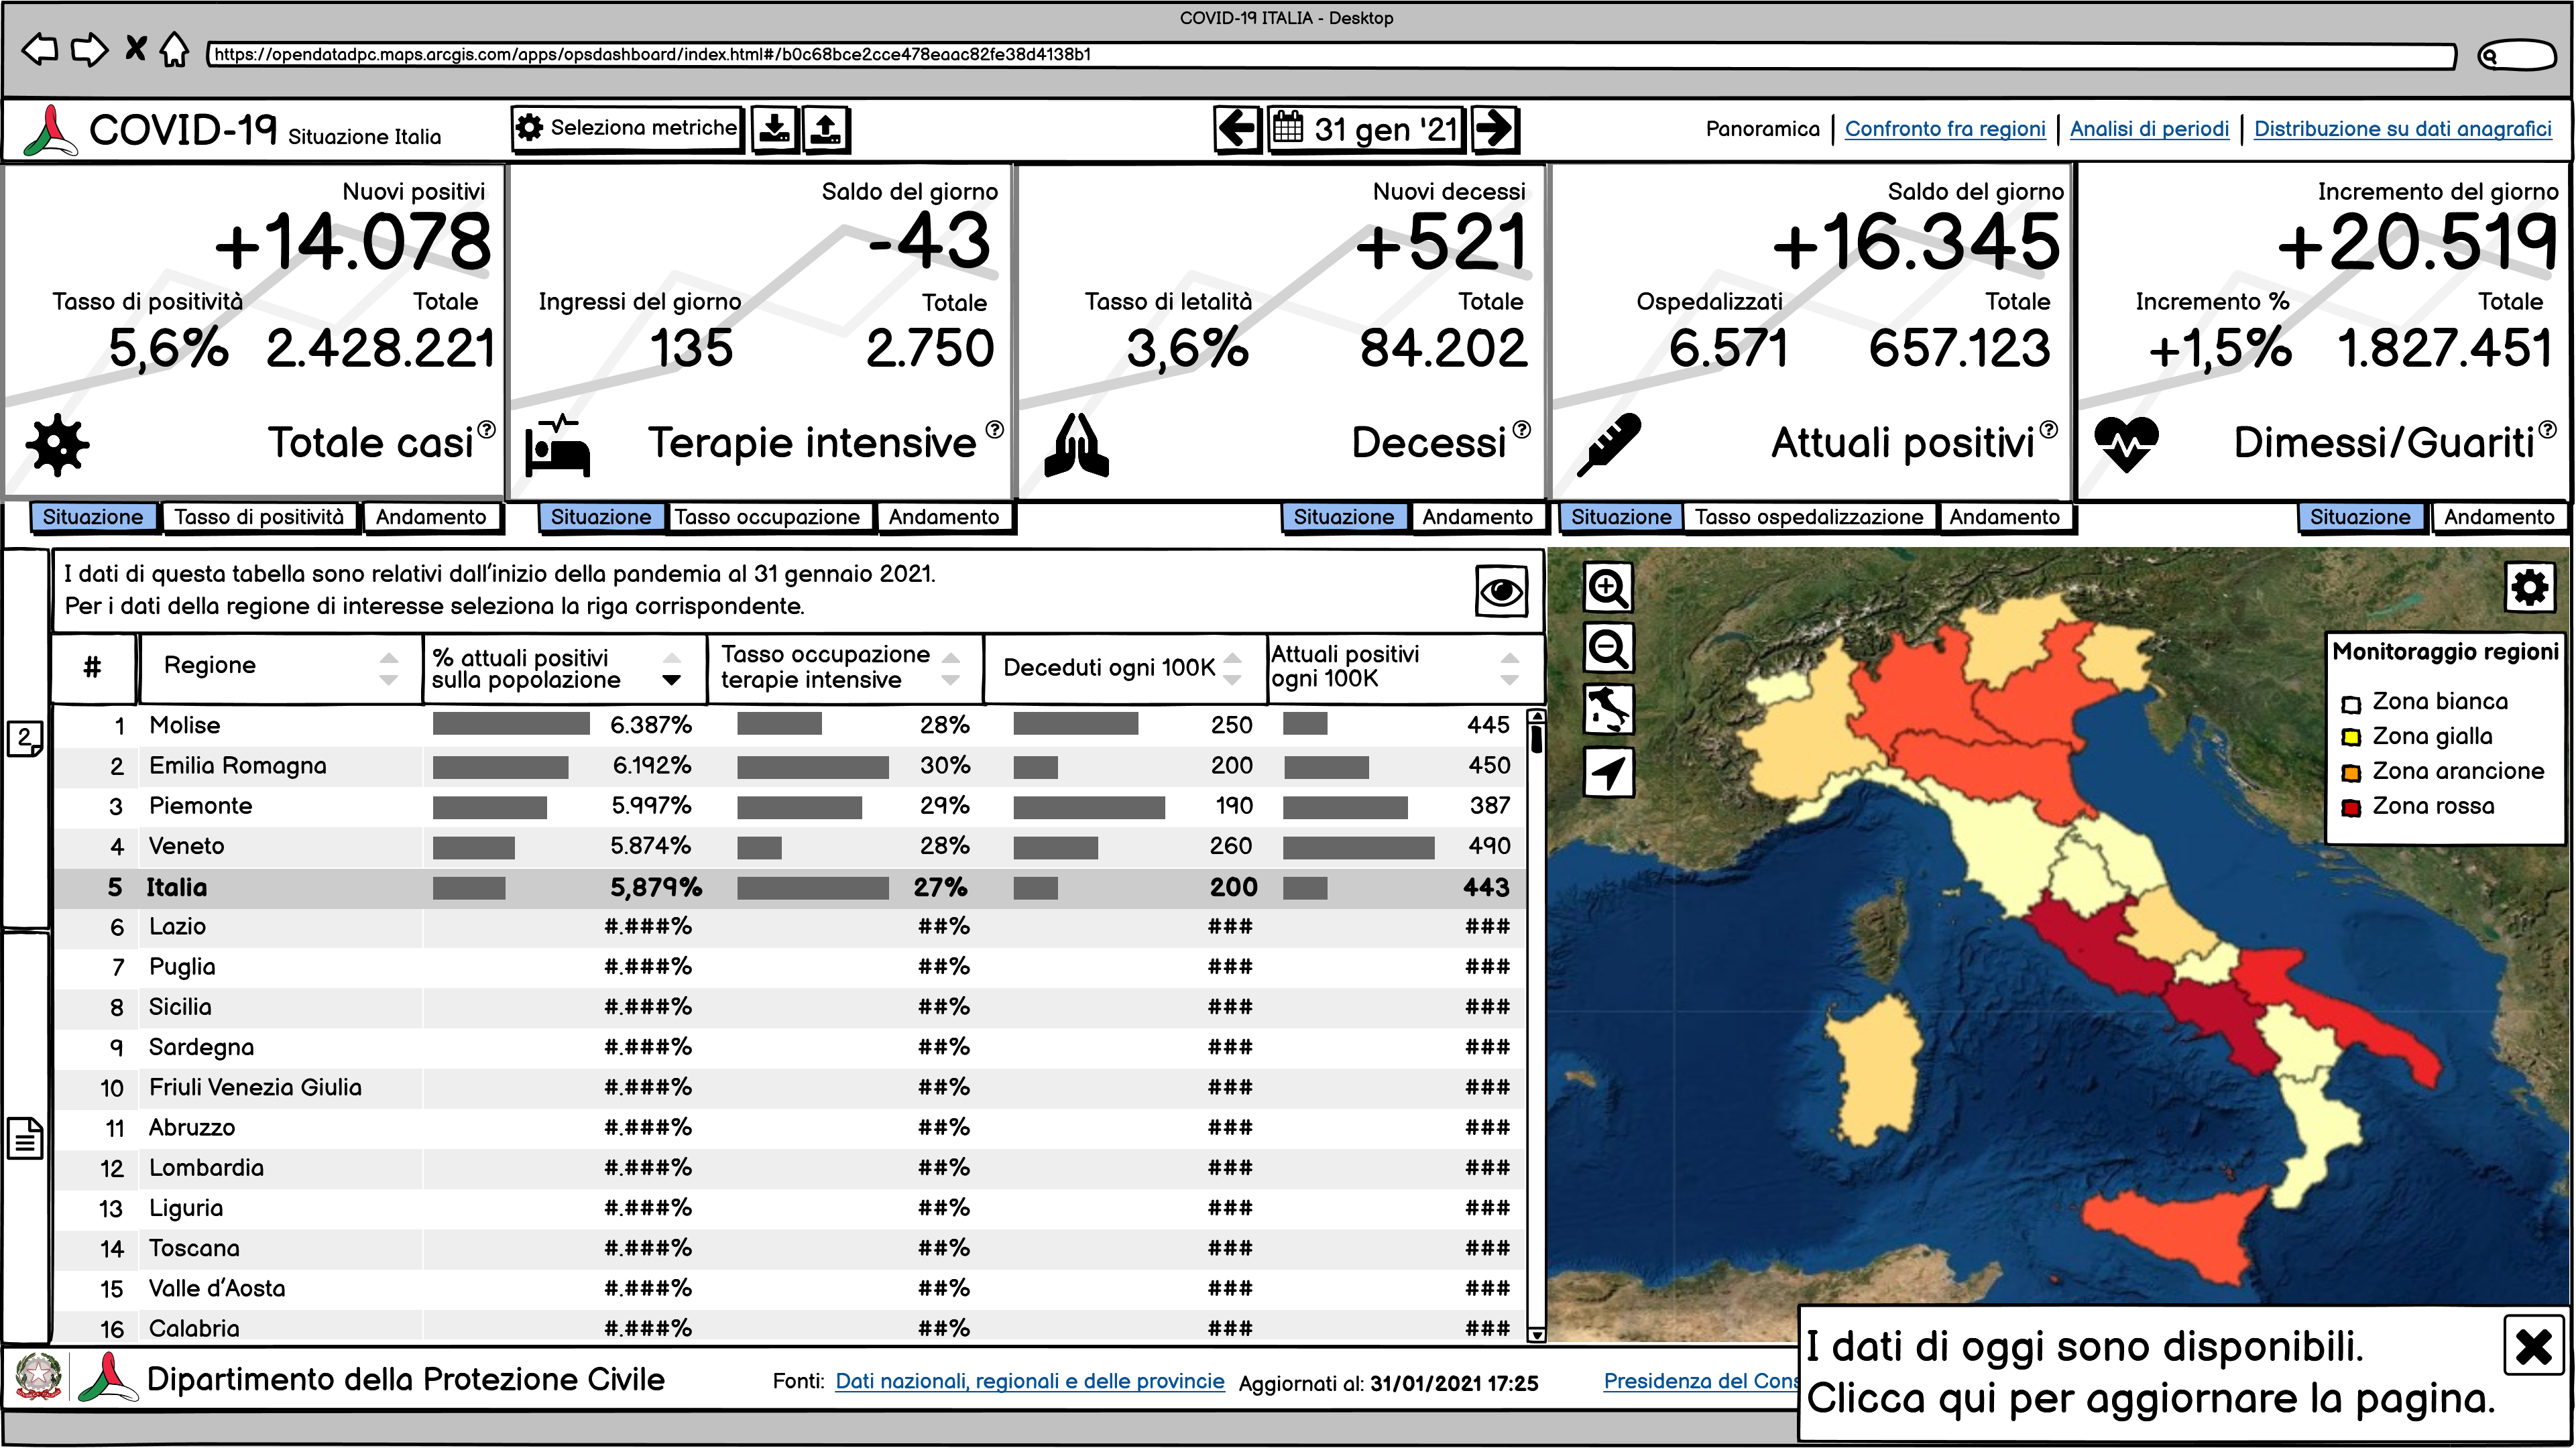
\includegraphics[trim = 800 0 0 310, clip, width=\columnwidth]{screen-interfaccia/Panoramica (pop-up aggiornamento dati)}
            \caption{Esempio della comparsa del pop-up di aggiornamento.}
        \end{figure}

    \end{columns}

    

\end{frame}